\section{FORS+C}
FORS (Forest of Random Subsets) is a few-time signature scheme used at the bottom of the stateless hypertree. FORS allows to sign a limited number of messages, when the security degrades with each use. Standard FORS signs a message by revealing \texttt{k} secret values, one from each of \texttt{k} binary trees of height \texttt{a}. The message digest determines which leaf to reveal from each tree. FORS+C applies the same checksum grinding optimization as WOTS+C to reduce signature size.

\subsection{FORS Structure}
FORS consists of \texttt{k} binary trees, each of height \texttt{a}:
\begin{itemize}
    \item Each tree has \texttt{2\^a} leaves
    \item Each leaf is derived from \texttt{SK.seed} using PRF
    \item The message digest is split into \texttt{k} chunks of \texttt{a} bits each
    \item Each chunk selects one leaf index from the corresponding tree
\end{itemize}
\begin{figure}[h!]
    \centering
    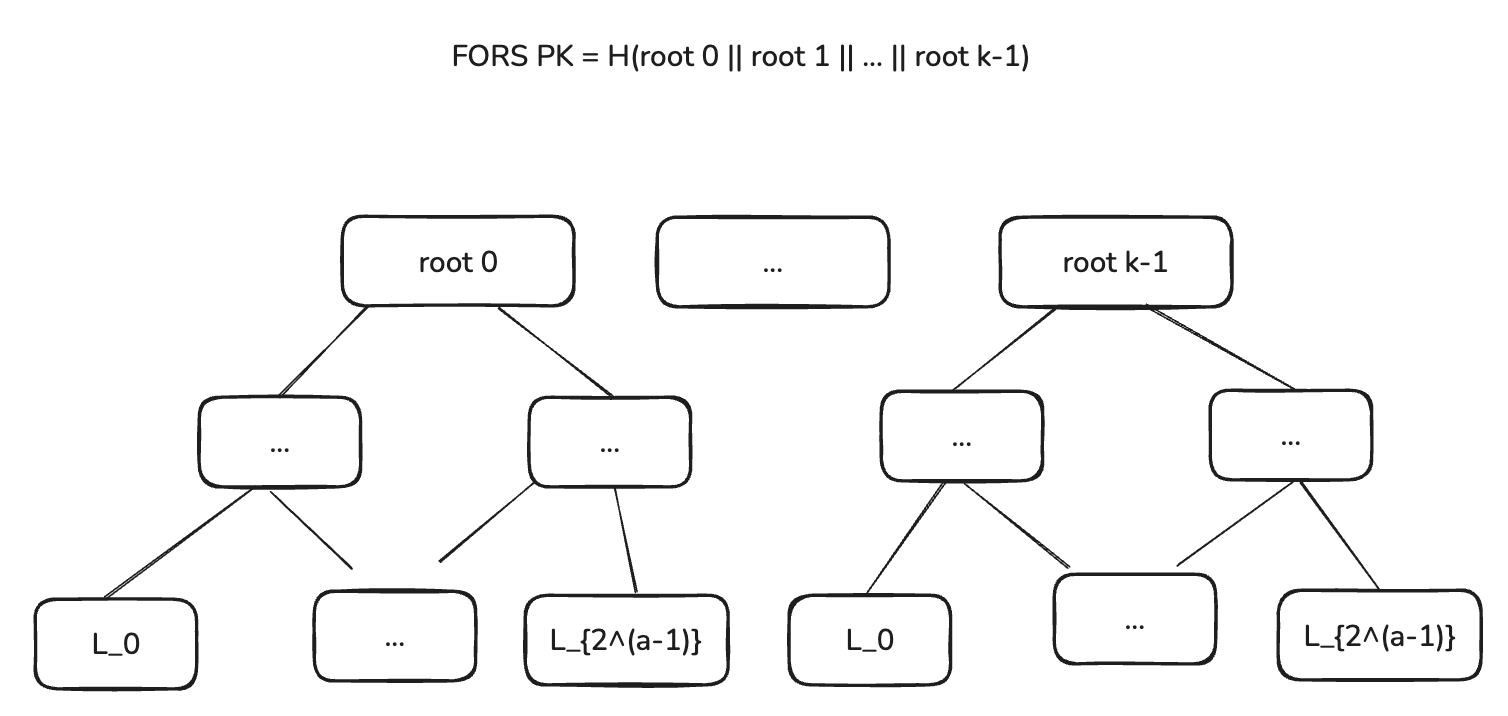
\includegraphics[width=0.8\linewidth]{content/img/fors.png}
    \caption{FORS architecture}
    \label{fig:shrincs}
\end{figure}

\subsection{Grinding Condition}
\begin{verbatim}
    digest = H_msg(ADRS, R, ctr, PK.seed, PK.root, m)
    condition: digest[last a bits] == 0 
\end{verbatim}

Cost is expected to be $\approx 2^a$ iterations.

\subsection{Message to Indices}
\begin{verbatim}
    Algorithm: fors_msg_to_indices(digest)
    Input:
        digest: message digest
    Output:
        indices: array of k integers in [0, 2^a - 1]

    1. indices ← []
    2. for i from 0 to k - 1:
        a. indices[i] ← extract_bits(digest, i × a, a)
    3. return indices
\end{verbatim}

\subsection{Grinding}
\begin{verbatim}
    Algorithm: fors_grind(m, R, PK.seed, PK.root, ADRS)
    Input:
        m: message to sign
        R: randomness
        PK.seed: public seed
        PK.root: public key root
        ADRS: tweak
    Output:
        indices: array of k integers
        ctr: counter value

    1. setTypeAndClear(ADRS, H_MSG)
    2. for ctr from 0 to 2^32 - 1:
        a. digest ← H_msg(ADRS, R, ctr, PK.seed, PK.root, m)
        b. indices ← fors_msg_to_indices(digest)
        c. if indices[k-1] == 0:
            return (indices, ctr)
    3. abort with error
\end{verbatim}

\subsection{Secret Key Generation}
\begin{verbatim}
    Algorithm: fors_SKgen(SK.seed, PK.seed, ADRS, tree_idx, leaf_idx)
    Input:
        SK.seed: secret seed
        PK.seed: public seed
        ADRS: tweak
        tree_idx: tree index (0 to k-1)
        leaf_idx: leaf index within tree
    Output:
        sk: secret value (n bytes)

    1. setTypeAndClear(ADRS, PRF)
    2. setKeyPairAddress(ADRS, tree_idx)
    3. setTreeIndex(ADRS, leaf_idx)
    4. sk ← PRF(PK.seed, ADRS, SK.seed)
    5. return sk
\end{verbatim}

\subsection{TreeHash}
\begin{verbatim}
    Algorithm: fors_treehash(SK.seed, PK.seed, ADRS, tree_idx, target_height, start_idx)
    Input:
        SK.seed, PK.seed: seeds
        ADRS: tweak
        tree_idx: tree index (0 to k-1)
        target_height: height of output node
        start_idx: leftmost leaf index in subtree
    Output:
        node: hash value (n bytes)

    1. if target_height == 0:
        a. sk ← fors_SKgen(SK.seed, PK.seed, ADRS, tree_idx, start_idx)
        b. setTypeAndClear(ADRS, SL_FORS)
        c. setKeyPairAddress(ADRS, tree_idx)
        d. setTreeHeight(ADRS, 0)
        e. setTreeIndex(ADRS, start_idx)
        f. return Tw(PK.seed, ADRS, sk)
    2. left ← fors_treehash(SK.seed, PK.seed, ADRS, tree_idx, target_height-1, start_idx)
    3. right ← fors_treehash(SK.seed, PK.seed, ADRS, tree_idx, target_height-1, start_idx + 
                2^(target_height-1))
    4. setTypeAndClear(ADRS, SL_FORS)
    5. setKeyPairAddress(ADRS, tree_idx)
    6. setTreeHeight(ADRS, target_height)
    7. setTreeIndex(ADRS, start_idx >> target_height)
    8. return Tw(PK.seed, ADRS, left || right)
\end{verbatim}

\subsection{FORS Authentication path}
\begin{verbatim}
    Algorithm: fors_auth_path(SK.seed, PK.seed, ADRS, tree_idx, leaf_idx)
    Input:
        SK.seed, PK.seed: seeds
        ADRS: tweak
        tree_idx: tree index (0 to k-1)
        leaf_idx: leaf index being revealed
    Output:
        auth: authentication path (a × n bytes)

    1. auth ← []
    2. for h from 0 to a - 1:
        a. sibling_start ← (leaf_idx XOR 2^h) AND (0xFFFFFFFF << h)
        b. auth ← auth || fors_treehash(SK.seed, PK.seed, ADRS, tree_idx, h, sibling_start)
    3. return auth
\end{verbatim}

\subsection{Signature generation}
\begin{verbatim}
    Algorithm: fors_sign(m, SK.seed, SK.prf, PK.seed, PK.root, ADRS)
    Input:
        m: message
        SK.seed: secret seed
        SK.prf: PRF key
        PK.seed: public seed
        PK.root: public key root
        ADRS: tweak
    Output:
        sig: FORS+C signature

    1. opt_rand ← random(n) or PK.seed
    2. R ← PRF_msg(SK.prf, PK.seed, opt_rand, m)
    3. (indices, ctr) ← fors_grind(m, R, PK.seed, PK.root, ADRS)
    4. sig ← R || toByte(ctr, c)
    5. for i from 0 to k - 2:
        a. sk_i ← fors_SKgen(SK.seed, PK.seed, ADRS, i, indices[i])
        b. auth_i ← fors_auth_path(SK.seed, PK.seed, ADRS, i, indices[i])
        c. sig ← sig || sk_i || auth_i
    6. sk_last ← fors_SKgen(SK.seed, PK.seed, ADRS, k-1, 0)
    7. root_last ← fors_treehash(SK.seed, PK.seed, ADRS, k-1, a, 0)
    8. sig ← sig || sk_last || root_last
    9. return sig
\end{verbatim}

\subsection{Public Key Recovery}
\begin{verbatim}
    Algorithm: fors_pkFromSig(sig, m, PK.seed, PK.root, ADRS)
    Input:
        sig: FORS+C signature
        m: message
        PK.seed: public seed
        PK.root: public key root
        ADRS: tweak
    Output:
        pk: FORS public key (n bytes), or $\bot$ if invalid

    1. R ← sig[0 : R_SIZE]
    2. ctr ← sig[R_SIZE : R_SIZE + c]
    3. setTypeAndClear(ADRS, H_MSG)
    4. digest ← H_msg(ADRS, R, ctr, PK.seed, PK.root, m)
    5. indices ← fors_msg_to_indices(digest)
    6. if indices[k-1] != 0:
        return $\bot$

    7. roots ← []
    8. offset ← R_SIZE + c
    9. for i from 0 to k - 2:
        a. sk_i ← sig[offset : offset + n]
        b. auth_i ← sig[offset + n : offset + n + a × n]
        c. offset ← offset + n + a × n
        d. setTypeAndClear(ADRS, SL_FORS)
        e. setKeyPairAddress(ADRS, i)
        f. setTreeHeight(ADRS, 0)
        g. setTreeIndex(ADRS, indices[i])
        h. node ← Tw(PK.seed, ADRS, sk_i)
        i. idx ← indices[i]
        j. for h from 0 to a - 1:
            setTreeHeight(ADRS, h + 1)
            setTreeIndex(ADRS, idx >> 1)
            if (idx AND 1) == 0:
                node ← Tw(PK.seed, ADRS, node || auth_i[h × n : (h+1) × n])
            else:
                node ← Tw(PK.seed, ADRS, auth_i[h × n : (h+1) × n] || node)
            idx ← idx >> 1
    k. roots[i] ← node
    10. sk_last ← sig[offset : offset + n]
    11. root_last ← sig[offset + n : offset + 2 × n]
    12. roots[k-1] ← root_last
    13. setTypeAndClear(ADRS, SL_FORS)
    14. setTreeHeight(ADRS, a)
    15. setTreeIndex(ADRS, 0)
    16. pk ← Tw(PK.seed, ADRS, roots[0] || ... || roots[k-1])
    17. return pk
\end{verbatim}